\documentclass[11pt, oneside]{article}   	% use "amsart" instead of "article" for AMSLaTeX format
\usepackage{geometry}                		% See geometry.pdf to learn the layout options. There are lots.
\geometry{letterpaper}                   		% ... or a4paper or a5paper or ...
%\geometry{landscape}                		% Activate for rotated page geometry
%\usepackage[parfill]{parskip}    		% Activate to begin paragraphs with an empty line rather than an indent
\usepackage{graphicx}				% Use pdf, png, jpg, or eps§ with pdflatex; use eps in DVI mode
								% TeX will automatically convert eps --> pdf in pdflatex
\usepackage[bb=boondox]{mathalfa}
\usepackage{mathtools}
\usepackage{amssymb}
\usepackage{amsmath,amsfonts,amsthm} % Math packages
\usepackage{bm}
\usepackage{graphicx}
\usepackage{dsfont}
\graphicspath{ {images/} }

%SetFonts

%SetFonts

\DeclareMathOperator*{\argmin}{arg\,min}
\DeclareMathOperator*{\argmax}{arg\,max}
\newcommand{\horrule}[1]{\rule{\linewidth}{#1}} % Create horizontal rule command with 1 argument of height

\title{
\normalfont \normalsize
\textsc{14D006 Stochastic Models and Optimization} \\ [25pt] % Your university, school and/or department name(s)
\horrule{0.5pt} \\[0.4cm] % Thin top horizontal rule
\huge Play Selection in American Football\\ % The assignment title
\horrule{2pt} \\[0.5cm] % Thick bottom horizontal rule
}

\author{Daniel Bestard, Michael Cameron, Hans-Peter H{\"o}llwirth, Akhil Lohia} % Your name

\date{\normalsize\today} % Today's date or a custom date

\begin{document}

\maketitle

%%%%%%%%
% Motivation %
%%%%%%%%
\section{Motivation}
We consider the dynamic programming framework to compute an optimal policy for play choice in an American football game for one drive from the view of the offensive team. In this context, the policies refer to the different plays an offensive team can make at each game situation. At every field position, the aim of the team is to choose among different possible options (run, pass, kick or punt) such that the expected reward is maximized. The reward is defined as the difference in number of points received at the end of the team's possession and the anticipated points of the opposition from our final field position. \\

We consider policy iteration algorithms for this task. The large number of possible states in the system (15,250), makes it hard to find the optimal solution numerically. Instead, we consider neuro-dynamic programming algorithms which approximate the optimal solution. In particular, we apply Approximate Policy Iteration (API) and Optimistic Policy Iteration (OPI) to estimate the reward-to-go function from simulated sample drives.\\

The project is based on the paper "Play Selection in American Football: A Case Study in Neuro-Dynamic Programming" by Patek and Bertsekas (1997). In the following sections we assume some basic understanding of the American football rules.


%%%%%%%%%%%%
% The Football Model %
%%%%%%%%%%%%
\section{The Football Model}
In our American football model we consider the score of one offense drive and add to it the expected points gained by the opposing team from our final field position. More concretely, we want to maximize the expected difference between our drive-score and the opposing team's responding drive-score (which is simply a function of our final field position). We now introduce the elements used by the dynamic programming algorithms to solve the optimization problem. \\\\
The \textbf{state} of the system $i \in S$ is described by a vector of 3 quantities: $i = [x,y,d]$:
\begin{itemize}
\item x = the number of yards to the opposition goal line (discrete value between 1 and 100)
\item y = the number of yards to go until the next first down (discrete value between 1 and 100)
\item d = down number ($\in \{1,2,3,4\}$)
\end{itemize}

\begin{figure}[ht!]
\centering
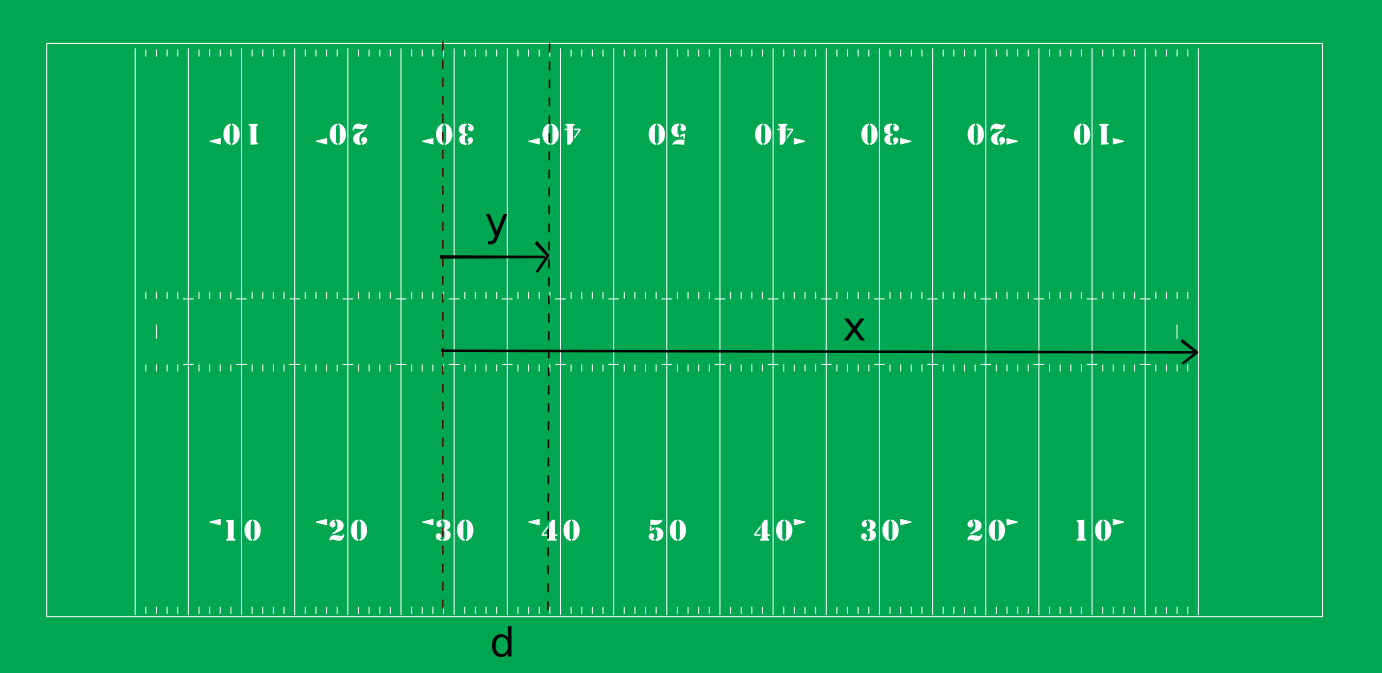
\includegraphics[width=155mm]{../images/field.png}
\caption{Illustration of state}
\end{figure}

At each state, the team can choose from one of 4 play options (\textbf{actions}) $u \in U$ with $U=\{R, P, U, K\}$. Each play is described using probability distributions, to model the yards gained. For this section we use the models set out in the original paper:
\begin{itemize}
\item (R)un: moves $D_p - 2$ yards forward with $D_p \sim \text{Poisson}(6)$, with probability 0.05 of a fumble.
\item (P)ass: moves $D_p - 2$ yards forward with $D_p \sim \text{Poisson}(12)$, with probability 0.05 of an interception, 0.45 of incompletion, 0.05 of quarterback sack and 0.45 of completion.
\item P(U)nt: moves $6 D_p  + 6$ yards forward with $D_p \sim \text{Poisson}(10)$
\item (K)ick: successful with probability $\max(0, .95 - .95x/60)$
\end{itemize}
The set of state-action pairs determine the stationary \textbf{policy} $\mu$. We look to choose the policy at any given state to maximise the expected reward. The \textbf{reward} of the drive is determined by the final state transition:
\begin{itemize}
\item Touchdown: 6.8 points (from run or pass)
\item Opponent's touchdown: -6.8 points (from run or pass)
\item Safety: -2.0 points (from pass or run)
\item Field goal: 3.0 points (from kick)
\item No score due to fumble (from run), interception (from pass), missed 4th down (from pass or run), missed field-goal (from kick) or punt
\end{itemize}

\subsection{Example}
A drive might look like as follows:
$$
\begin{bmatrix} 25\\[0.3em] 10 \\[0.3em] 1 \end{bmatrix}
\longrightarrow_0^P
\begin{bmatrix} 17\\[0.3em] 2 \\[0.3em] 2 \end{bmatrix}
\longrightarrow_0^R
\begin{bmatrix} 14\\[0.3em] 10 \\[0.3em] 1 \end{bmatrix}
\longrightarrow_0^P
\begin{bmatrix} 10\\[0.3em] 6 \\[0.3em] 2 \end{bmatrix}
\longrightarrow_0^P
\begin{bmatrix} 10\\[0.3em] 6 \\[0.3em] 3 \end{bmatrix}
\longrightarrow_0^R
\begin{bmatrix} 8\\[0.3em] 4 \\[0.3em] 4 \end{bmatrix}
\longrightarrow_3^K
T
$$
In this case, we start from field position $i^* = (x=25, y=10, d=1)$, i.e. with a first-down 25 yards from the endzone. The policy dictates to use a (P)ass play for this particular status which in this realization yields a 8 yard improvement, thus transitioning to $i^1 = (x=17, y=2, d=2)$. We continue with a mix of (P)ass and (R)un games and eventually (K)ick a field-goal at $4^{th}$-down which terminates the drive and results in a reward of 3 points.


%%%%%%%%%%%%%%%%%%%%
% Dynamic Programming Formulation %
%%%%%%%%%%%%%%%%%%%%
\newpage
\section{Dynamic Programming Formulation}
In this model of the football problem, the solution can be computed directly. However, the problem can quickly become computationally infeasible when introducing other elements of the game, such as time or half yard intervals.

%% comment: optimal solution not implemented. should be written as motivation for approximation solution!!
\subsection{Optimal Solution}
Our original problem has 15250 states. The rules of our model are such that at each first down there is a unique value of y associated with each value of x. Note, that the number of possible combinations is much larger than the 15250 that we claim. There is the additional constraint that it is impossible to have the number of yards to next down greater than yards to the goal line, that is, we cannot have $y>x$. This reduces the number of tates to 15250.\\

This is still a large problem. In their paper, Bertsekas and Patek, have carried out the computations to find the optimal policy. They have applied the dynamic programming algorithm.
$$
\mu^{k}(i) = arg\max\limits_{u \in U} \Big[ \sum\limits_{j \in S} p_{ij}(u)(g(i,u,j) +  J^{\mu^{k-1}}(j))\Big] \quad \forall i \in S
$$
This algorithm chooses the policy u  which maximises the expected reward. In the formula above, $i$ represents the state we are currently in and $j$ is the state we move to. $p_{ij}(u)$ are the transition probabilities, giving the probability from moving from state $i$ to state $j$ under action $u$. The reward function is $g(i,u,j)$, which is 0 in every stage except for the terminal state. This is because we only gain rewards after scoring or losing the ball. While $J^{\mu^{k-1}}(j)$ is the reward-to-go  function from the state $j$. \\

Using this exact method we obtain an optimal policy for any state of the 4 downs. These optimal policies can be seen in Figure 1,1 in Bertsekas and Patek. As a benchmark, using this policy from the state $(x,y,d)=(80,10,1)$ (a common starting point in football) and running simulations with the optimal policy, the expected net reward is -0.9449 points. This means that if we start each drive in this state, we are expected to lose the game! \\

Although, this problem is computationally possible. It is still a large problem and can easily be made even bigger by introducing other variables, such as time. This is the basis for our motivation to use approximations to compute the optimal policies. Using these approximation methods it is possible to go on to compute larger problems, whereas finding the exact solution becomes computationally unfeasible easily.



\subsection{Approximation with Neuro-Dynamic Programming}
An important part of the implentation of this algorithm is the apporximations of the reward-to-go functions. We aim to calculate the approximate reward-to-go function for fixed policies, we can then focus on computing new policies given these approximations. Given the approximation $\widetilde{J}(i,r^{k-1})$ for a stationary policy $\mu^{k-1}$, compute a new policy $\mu^{k}$ by
$$
\mu^{k}(i) = G(r)(i) = arg\max\limits_{u \in U} \Big[ \sum\limits_{j \in S} p_{ij}(u)(g(i,u,j) +  \widetilde{J}(i,r^{k-1}))\Big] \quad \forall i \in S
$$
This is very similar to the dynamic programming algorithm we had seen previously, but now we are using the approximations. \\

To obtain these approximations, we first run many simulated drives. Each drive will produce a reward given a randomly assigned starting position. This acts as our data to train the architecture of our approximation model. The architecture can take different forms. For instance Multi-Layered Perceptron (MLP), where a neural network is trained to give the approximate reward-to-go function, given a state. This is the method we implement in this report, but other frameworks are possible, such as the Quadritic architecture or Quadratic with Feature. More information on these two architectures can be found in the original Bertsekas and Patek paper.

%%%%%%%%
% Simulation %
%%%%%%%%
\section{Simulation}
The approximations of the reward-to-go function $J_{u_k}(i^*)$ are obtained from simulated sample trajectories. The simulation routine takes as inputs a policy $\mu$ and a starting state $i^*$ and then generates $N$ sample drives. Each generated sample drive represents a realization of the following probabilistic model (probabilities in brackets):
\begin{itemize}
\item (R)un attempts result in either
\begin{itemize}
\item (0.05) fumble
\item (0.95) run with movement $D_r -2$ with $D_r \sim \text{Poisson}(6)$
\end{itemize}
\item (P)ass attempts result in either
\begin{itemize}
\item (0.05) pass interception with movement $D_p -2$ with $D_p \sim \text{Poisson}(12)$
\item (0.05) sack with movement $D_s$ with $D_s \sim \text{Poisson}(6)$
\item (0.45) pass incomplete
\item (0.45) pass complete with movement $D_p -2$ with $D_p \sim \text{Poisson}(12)$
\end{itemize}
\item P(U)nt attempts always result in turn-over with movement $6 D_p + 6$ with $D_p \sim \text{Poisson}(10)$
\item (K)ick attempts result in either
\begin{itemize}
\item (max(0,(0.95-0.95x/60)) successful field goal
\item (otherwise) missed field goal
\end{itemize}
\end{itemize}
No reward is earned in any state transition, except for the case where the drive terminates. The drive terminates in any of the following events:
\begin{itemize}
\item touchdown (reward: 6.8)
\item successful field-goal (reward: 3.0)
\item missed field-goal, punt, fumble, interception, missed $4^{th}$-down (reward: 0.0)
\item safety (reward: -2.0)
\item opponent's touchdown (=interception in opponent's endzone) (reward: -6.8)
\end{itemize}
Once the drive is terminated, the final field position $x$ of the drive determines the expected points gained by the opposing team: $6.8x/100$.
The simulation returns $N$ such sample drives. Each drive $l$ is described by its status sequence $(i_t^l)$ for $t=1,...,T^l$ and reward $g_{T^i}^l$.

\subsection{Expected Reward}
Given a set of $N$ simulated sample trajectories for a specific policy $\mu$, we can estimate the expected reward of this policy from a starting state $i^*$:
$$
\widetilde{J}_{u_k}(i^*) = \frac{1}{N}\sum_{l=1}^N g_{T^i}^l
$$
where $g_{T^i}^i$ denotes the reward of the $i^{th}$ sample trajectory with drive length $T^i$.

\subsection{Heuristic Benchmark}
The simulations and the expected reward function can be used to yield a heuristic benchmark for the optimal play-selection policy. We use the suggested heuristic policies from the paper in order to establish the correctness of the simulation algorithm. In particular, we consider the following heuristic policies:
\begin{enumerate}
\item If $d=1$ (first down): (\textbf{P})ass

\item If $d=2$ (second down):
\begin{enumerate}
\item If $y<3$ (less than 3 yards to next first down): (\textbf{R})un
\item If $y\geq3$ (3 or more yards to next first down): (\textbf{P})ass
\end{enumerate}

\item If $d=3$ (third down):
\begin{enumerate}
\item If $x<41$ (less than 41 yards to goal):
\begin{enumerate}
\item If $y<3$ (less than 3 yards to next first down): (\textbf{P})ass or (R)un
\item If $y\geq3$ (3 or more yards to next first down): (\textbf{P})ass or (R)un
\end{enumerate}
\item If $x \geq 41$ (less than 41 yards to goal):
\begin{enumerate}
\item If $y<3$ (less than 3 yards to next first down): (P)ass or (\textbf{R})un
\item If $y\geq3$ (3 or more yards to next first down): (\textbf{P})ass or (R)un
\end{enumerate}
\end{enumerate}

\item If $d=4$ (forth down):
\begin{enumerate}
\item If $x<41$ (less than 41 yards to goal):
\begin{enumerate}
\item If $y<3$ (less than 3 yards to next first down): (P)ass or (\textbf{R})un or (K)ick
\item If $y\geq3$ (3 or more yards to next first down): (P)ass or (R)un or (\textbf{K})ick
\end{enumerate}
\item If $x \geq 41$ (less than 41 yards to goal):
\begin{enumerate}
\item If $y<3$ (less than 3 yards to next first down): (P)ass or (\textbf{R})un or P(U)nt
\item If $y\geq3$ (3 or more yards to next first down): (P)ass or (R)un or P(\textbf{U})nt
\end{enumerate}
\end{enumerate}

\end{enumerate}

We estimated the expected reward for each of the $2^4*3^4 = 1296$ heuristic policy combinations from starting position $i^* = (x=80, y=10, d=1)$ (one of the most likely starting positions in football) and found the best heuristic expected reward-to-go $J_{\mu}(i^*) = -1.26$. The associated policy to this reward is highlighted in bold. Note that the reward-to-go matches the heuristic result of the underlying paper, thus establishing the correctness of the simulation algorithm.

%%%%%%%%%
% API and OPI %
%%%%%%%%%
\section{Approximate and Optimistic Policy Iteration}
The aim now is to approximate the reward-to-go function to be used in the policy update algorithm, We have two different approaches to this problem, API and OPI. In API, we run many drive simulations over few different policies. In contrast, for OPI, we run much fewer simulations per iteration, but need more iterations to converge to a good policy choice.\\

We now describe in detail how the algorithms API and OPI are implemented in practice. Let $N_{p}$, $N_{e}$ , $N_{s}$ and $N_{t}$ denote the parameters of the algorithm which are set by the user in advance. Even thought the definition of these parameters can be inferred from the algorithm, it is more clear to define them separately:
\begin{itemize}
    \item $N_{p}$: if, for example, $N_{p}=20$, then in every 20th iteration we compute the expected reward-to-go.
    \item $N_{e}$: number of sample trajectories that we use to compute the estimate of the reward-to-go function.
    \item $N_{s}$: number of sample trajectories in the in training set $D_{k}$ (see later).
    \item $N_{t}$: maximum number of training cycles for neural network.
\end{itemize}
The implementation of the algorithm is as follows:
\begin{enumerate}
    \item Start with an initial policy $\mu_{0}$.
    \item Iteratively compute
    \begin{enumerate}
    \item Given $\mu_{k}$, if $k \in \{j \cdot N_{p} | j=0,1,2,…\}$, then generate $N_{e}$ sample trajectories, each starting from $i^{*}$, to obtain an estimate of $J_{\mu_{k}}(i^{*})$
    \item Given the probabilistic rule for picking initial conditions, generate $N_{s}$ sample trajectories and record $D_{k}$, where the last element is simply an object that stores the reward and the sequence of the vector of states. $D_{k}$ is created because we use its elements in the next step of the algorithm.
    \item We fit the neural networks to estimate the reward-to-go function and save the object in a variable that we call $r^{k}$ which uses the elements of $D_{k}$. The neural networks cycle through the data $N_{t}$ times.
    \item Compute a new policy $\mu_{k+1} := G(r^{k})$, where $G$ is the “greedy” operator which chooses the actions at each state that are best with respect to the reward-to-go approximation given by $r^{k}$.
    \end{enumerate}
\end{enumerate}
We set $\mu_{0}$ to an heuristic policy. Step (a) and the underlying simulation function are described in chapter 4.

\subsection{Generating Sample Drives}
At each iteration we generate $N_S$ sample drives by simulation. In contrast to the sample simulation for estimating the expected reward, we choose the initial state of the drive randomly. The random mechanism ensures that we encounter the most likely states with high probability. The mechansim looks as follows:
%% Add sampling initial conditions
\begin{enumerate}
\item Set $d=1$ (first down) with probability 0.10
\begin{itemize}
\item With probability 0.25 $x$ is chosen uniformly from 1 to 75.
\item With probability 0.75 $x$ is chosen uniformly from 76 to 100.
\item If $x < 10$ ,choose $y=x$. Else choose $y=10$
\end{itemize}
\item Set $d=2$ (second down) with probability 0.25
\begin{itemize}
\item With probability 0.25 $x$ is chosen uniformly from 1 to 50.
\item With probability 0.75 $x$ is chosen uniformly from 51 to 100.
\item Yards to next first down, $y$, is chosen uniformly from 1 to x.
\end{itemize} 
\item Set $d=3$ (third down) with probability 0.30
\begin{itemize}
\item Yards to go to goal line, $x$, is chosen uniformly from 1 to 100.
\item Yards to next first down, $y$, is chosen uniformly from 1 to x.
\end{itemize}
\item Set $d=4$ (fourth down) with probability 0.35
\begin{itemize}
\item Yards to go to goal line, $x$, is chosen uniformly from 1 to 100.
\item Yards to next first down, $y$, is chosen uniformly from 1 to x.
\end{itemize}
\end{enumerate}

\subsection{Multilayer Perceptron (MLP)}
In our implementation, we use the multilayer perceptron (MLP) architecture to approximate the reward-to-go function $J_{\mu}(i)$ for policy $\mu$ from state $i$. We train 4 neural networks, one for each possible down $d$. Each neural network consists of 2 input nodes (scaled $x$ and $y$: ), one hidden layer with 20 nodes, and one output node ($J$). The architecture is depicted in figure 1. We scale the input values by a factor of $\sigma_{d}^{x} = \sigma_{d}^{y} = 0.01$ for all $d$ to obtain values in the range $[0,1]$. The neural networks then essentially find the least-squares estimates to the reward-to-go values $J_{\mu}(i)$. We use the R library \textit{nnet} to train the neural networks. The number of training cycles is limited to $N_t$. \\

The trained neural networks will then be used to predict the reward-to-go values for all possible states $i = (x,y,d)$. We compute the predictions for all state combinations and store them for the policy update step.


\begin{figure}[ht!]
\centering
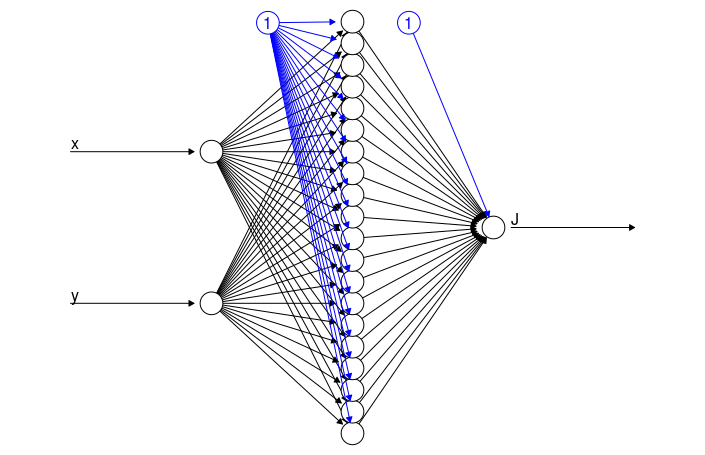
\includegraphics[width=155mm]{../images/neuralnet.png}
\caption{Architecture of neural network with one hidden layer ($R=20$ nodes)}
\end{figure}

\subsection{Policy Update}
Finally, we use the predictions for the reward-to-go function $J_{\mu}(i)$ from the trained neural network $r^{k-1}$ to update the policy:
$$
\mu^{k}(i) = G(r)(i) = arg\max\limits_{u \in U} \Big[ \sum\limits_{j \in S} p_{ij}(u)(g(i,u,j) +  \widetilde{J}(i,r^{k-1}))\Big] \quad \forall i \in S
$$
We set the immediate reward function $g(i,u,j) = 0$ for all $(i, j)$ pairs reward is only earned at the termination of the drive. Furthermore, we take the estimates for the reward-to-go $\widetilde{J}(i,r^{k-1})$ from the neural network output.\\

To compute the expected reward, all that is left is finding the transition probabilities $p_{ij}(u)$ from state $i$ to state $j$ with action $u$. Note that the transition matrix $P(u) = (p_{ij}(u)$ is of dimension $15,250 \times 15,250$! Unfortunately, the paper does not mention how to derive the transition probabilities. We decided to use the generated sample data to empirically estimate the transition probabilities. Note that this approach gives us a sparse transition matrix, even for large sample sizes $N_S$. However, this sparsity allows us to compute the sum over all possible transitions effectively. \\

In a final step, we compare the expected reward of a state $i$ with each action $u \in \{P, R, U, K\}$ and set $\mu^k(i)$ to the action that gives the maximum expected reward.

%%%%%%
% Results %
%%%%%%
\section{Results}

The football case study provides an effective testbed to evaluate the NDP framework. We implement the API and OPI algorithms using the Multilayer Perceptron architecture. In this case, the multilayer perceptron basically boils down to a neural network with one hidden layer of 20 nodes.
The neural network trained on simulated drives from random starting points allow to approximate the reward-to-go from a given state instead of having to take a recursive path of calculating the expected reward. This is the major idea of the study which differentiates the reinforcement learning approach from usual dynamic programming.

The football model represents a challenge for the approximate methods and seems to have characteristics of truly large scale examples. Apart from that, since we know the optimal results, it allows to evaluate the performance of our model. Finally, football is intuitive. This aids in the implementation and de-bugging of the algorithms and also provides a means for interpreting the results.

\subsection{Heuristic Policy Results}
We evaluate a large set of heuristic policies from a given starting point to find the one which gives the best results based on a large number of simulated drives. The best heuristic policy gives an expected reward of -1.2653 which is about .3 points worse than the optimal results.

\subsection{API and OPI Results}
We try a wide range of number of samples and iterations to get the updated policies for a given starting point. Unfortunately we do not achieve a convergence in terms of the expected reward from the given starting state. We obtain noisy expected scores in the same ballpark as Patek and Bertsekas albiet with quite a bit of variation.
Possible ways we could think of to gain convergence include the following:
\begin{itemize}
	\item Continuously update the same neural network using new generated samples instead of training new models at every iteration. This should probably provide us with better approximates of the expected reward to go.
	\item The calculation of transition probabilities can be done in a more sophisticated manner. Since we know the probabilistic results of every action taken at a given state, we should be able to calculate the expected state to which we will transition instead of considering the possibilities of all possible transitions.
	\item We can modify the architecture of the model we use to approximate the reward to go from a given state. Currently we use a neural network with 1 hidden layer and 20 nodes. A deeper network with more layers or a different architecture like the quadratic or recursive one discussed by Patek and Bertsekas in their could result in less noisy approximate rewards from a given state.
\end{itemize}

\end{document}















